\lecture{5}{6 Oct.}{}

\begin{recall}
    A \vocab{tournament} \(T\) is an orientation of \(K_n\): for every pair of vertices exactly one of the arcs \((u,v)\), \((v,u)\) belongs to \(E(T)\), and we say \(u\) \vocab{beats} \(v\) if \((u,v) \in E(T)\). See \autoref{sec:schutte}.
\end{recall}

In \autoref{sec:sum-free} the first moment principle produced \emph{one} object of a given kind: a single large sum-free subset. The same principle also produces objects in \emph{quantity}: if the average number of copies of some structure is large, then some object contains at least that many copies. This section carries out the oldest example of this, which is also the oldest application of the probabilistic method at all.

\section{Hamilton Paths in Tournaments}\label{sec:hamilton-tournaments}

\subsection{Every Tournament Has One}

\begin{definition}[Hamilton path]\label{def:hamilton-path}
    Given a tournament \(T\) on \(n\) vertices \(v_1, \ldots, v_n\), a \vocab{Hamilton path} is a directed path that goes through every vertex exactly once, i.e.\ a sequence
    \[
        v_{\pi(1)}, v_{\pi(2)}, \ldots, v_{\pi(n)}, \qquad \text{where } (v_{\pi(i)}, v_{\pi(i+1)}) \in E(T) \ \forall\, 1 \le i < n \text{ and } \pi \in S_n.
    \]
\end{definition}

So a Hamilton path is an ordering of the players in which each one beats the next. Not every digraph has one; tournaments always do, because having \emph{all} pairs oriented leaves a vertex nowhere to hide.

\begin{claim}\label{clm:hamilton-exists}
    Every tournament has a Hamilton path.
\end{claim}

\begin{proof}
    A tournament is finite, so we may take a longest directed path
    \[
        P = v_1 \to v_2 \to \cdots \to v_t,
    \]
    and it suffices to show \(t = n\). Suppose not, and let \(v \notin P\).
    \begin{center}
        \begin{tikzpicture}[thick, >={Stealth[length=5pt]}, every node/.style={font=\small}]
            \foreach \i in {1,...,5} \coordinate (v\i) at (1.3*\i,0);
            \coordinate (v) at (3.9,1.5);
            \foreach \i [evaluate=\i as \j using int(\i+1)] in {1,...,4}
                \draw[->, shorten >=3pt, shorten <=3pt] (v\i) -- (v\j);
            \draw[->, red!80!black, shorten >=3pt, shorten <=3pt] (v1) to[out=60, in=180] (v);
            \foreach \i in {2,...,5}
                \draw[->, orange!85!black, shorten >=3pt, shorten <=3pt] (v\i) to[out=75, in=-60] (v);
            \foreach \i in {1,...,5} \fill (v\i) circle (2.2pt);
            \fill[blue!60!black] (v) circle (2.6pt);
            \node[above] at (v) {$v$};
            \foreach \i in {1,...,5} \node[below] at (v\i) {$v_{\i}$};
            \node[anchor=east] at (0.9,0) {$P$};
            \node[anchor=west, align=left] at (6.9,1.5)
                {first \(v_1\) must beat \(v\) (red),\\then so must every \(v_i\) (orange)};
        \end{tikzpicture}
    \end{center}
    \begin{itemize}
        \item If \((v, v_1) \in E(T)\), then \(v \to v_1 \to v_2 \to \cdots \to v_t\) is a longer path. Hence \((v_1, v) \in E(T)\).
        \item If \((v_i, v) \in E(T)\) for some \(i < t\), then \((v_{i+1}, v) \in E(T)\) as well: otherwise \((v, v_{i+1}) \in E(T)\), and
        \[
            v_1 \to \cdots \to v_i \to v \to v_{i+1} \to \cdots \to v_t
        \]
        is a longer path.
    \end{itemize}
    Starting from \((v_1, v) \in E(T)\) and applying the second item repeatedly gives \((v_t, v) \in E(T)\), so \(v_1 \to \cdots \to v_t \to v\) is a longer path. \conta
\end{proof}

Note that the proof shows more than existence: \emph{every} longest path is already a Hamilton path. The next example shows that the number of Hamilton paths can be as small as \(1\).

\begin{eg}[Transitive tournament]\label{eg:transitive}
    The \vocab{transitive tournament} on \(v_1, \ldots, v_n\) is the one with
    \[
        (v_i, v_j) \in E(T) \iff i < j,
    \]
    i.e.\ the players are linearly ranked and the better one always wins. It has a unique Hamilton path, namely \(v_1 \to v_2 \to \cdots \to v_n\): if \(v_{\pi(1)} \to \cdots \to v_{\pi(n)}\) is a Hamilton path, then \(\pi(i) < \pi(i+1)\) for every \(i\), so \(\pi\) is increasing, i.e.\ \(\pi = \id\).
    \begin{center}
        \begin{tikzpicture}[thick, >={Stealth[length=5pt]}, every node/.style={font=\small}]
            \foreach \i in {1,...,5} \coordinate (v\i) at (1.3*\i,0);
            \foreach \i [evaluate=\i as \j using int(\i+1)] in {1,...,4}
                \draw[->, blue!60!black, shorten >=3pt, shorten <=3pt] (v\i) -- (v\j);
            % the remaining arcs, all pointing forwards
            \draw[->, gray, shorten >=3pt, shorten <=3pt] (v1) to[out=45, in=135] (v3);
            \draw[->, gray, shorten >=3pt, shorten <=3pt] (v2) to[out=45, in=135] (v4);
            \draw[->, gray, shorten >=3pt, shorten <=3pt] (v3) to[out=45, in=135] (v5);
            \draw[->, gray, shorten >=3pt, shorten <=3pt] (v1) to[out=60, in=120] (v4);
            \draw[->, gray, shorten >=3pt, shorten <=3pt] (v2) to[out=60, in=120] (v5);
            \draw[->, gray, shorten >=3pt, shorten <=3pt] (v1) to[out=70, in=110] (v5);
            \foreach \i in {1,...,5} \fill (v\i) circle (2.2pt);
            \foreach \i in {1,...,5} \node[below=4pt] at (v\i) {$v_{\i}$};
            \node[anchor=west, align=left] at (7.2,0)
                {all arcs point to the right,\\so the only Hamilton path\\is the left-to-right one};
        \end{tikzpicture}
    \end{center}
\end{eg}

\subsection{Szele's Problem}

So one Hamilton path always exists, and sometimes there is exactly one. How many can there be?

\begin{question}[Szele, 1943]\label{q:szele}
    What is the maximum number of Hamilton paths an \(n\)-vertex tournament can have?
\end{question}

\begin{observation}\label{obs:n-factorial}
    Since a Hamilton path is specified by the ordering \(\pi \in S_n\) in which it visits the vertices, there are at most \(n!\) possible paths.
\end{observation}

\begin{definition}\label{def:P-n}
    Let \(P(n) = \max \{ \#\text{Hamilton paths in } T : T \text{ an } n\text{-vertex tournament} \}\).
\end{definition}

By \autoref{eg:transitive} and the observation above we have \(1 \le P(n) \le n!\), and the transitive tournament shows the lower bound is attained by \emph{some} tournament. The question is how large \(P(n)\) is, and this is where a random tournament comes in: no explicit construction is needed, because the average over all tournaments is already large.

\begin{proposition}[Szele, 1943]\label{prop:szele-lower}
    \(P(n) \ge \dfrac{n!}{2^{n-1}}\).
\end{proposition}

\begin{proof}
    Consider a uniformly random tournament \(T\) on the vertex set \([n]\): for every pair \(i \ne j\) we choose \((i,j)\) or \((j,i)\) uniformly at random, independently for each pair. Let
    \[
        X = \#\{\text{Hamilton paths in } T\}.
    \]
    For every permutation \(\pi \in S_n\), let \(E_\pi\) be the event that \(\pi(1), \pi(2), \ldots, \pi(n)\) is a Hamilton path of \(T\), and let \(X_\pi = \mathbbm{1}_{E_\pi}\). Every Hamilton path is counted by exactly one \(\pi\), so \(X = \sum_{\pi \in S_n} X_\pi\) and, by \autoref{thm:linearity},
    \[
        \mathbb{E}[X] = \sum_{\pi \in S_n} \mathbb{E}[X_\pi] = \sum_{\pi \in S_n} \mathbb{P}(E_\pi).
    \]
    Now
    \[
        E_\pi = \bigl\{ (\pi(1), \pi(2)) \in E(T) \bigr\} \cap \bigl\{ (\pi(2), \pi(3)) \in E(T) \bigr\} \cap \cdots \cap \bigl\{ (\pi(n-1), \pi(n)) \in E(T) \bigr\}
    \]
    is an intersection of \(n-1\) events about \(n-1\) \emph{distinct} pairs, which are independent and each of probability \(\frac{1}{2}\), so \(\mathbb{P}(E_\pi) = \bigl( \frac{1}{2} \bigr)^{n-1}\). Hence
    \[
        \mathbb{E}[X] = \sum_{\pi \in S_n} \mathbb{P}(E_\pi) = n! \cdot \Bigl( \frac{1}{2} \Bigr)^{n-1} = \frac{n!}{2^{n-1}},
    \]
    and by \autoref{lem:first-moment} some tournament \(T\) has \(X(T) \ge \mathbb{E}[X] = \frac{n!}{2^{n-1}}\) Hamilton paths.
\end{proof}

\begin{remark}\hfill
    \begin{enumerate}[(1)]
        \item The events \(E_\pi\) are heavily dependent --- two permutations can share many pairs --- and their number \(n!\) is enormous. Linearity does not care, exactly as in \autoref{eg:fixed-points}.
        \item Recall Stirling's formula \(n! \sim \sqrt{2\pi n} \bigl( \frac{n}{e} \bigr)^n\). So
        \[
            \frac{n!}{2^{n-1}} \sim 2\sqrt{2 \pi n} \Bigl( \frac{n}{2e} \Bigr)^n,
        \]
        which is still superexponentially large: a positive proportion \(2^{-(n-1)}\) of all \(n!\) conceivable orderings are realised simultaneously by one tournament.
        \item This is the first published use of the probabilistic method, predating Erd\H{o}s's lower bound for \(R(k)\) by four years. Note how little is proved about the good tournament \(T\): we never see it.
    \end{enumerate}
\end{remark}

Szele also proved an upper bound, \(P(n) \le \frac{n!}{2^{\frac{3}{4}(n-1)}}\), leaving a gap in the exponent between \(\frac{3}{4}(n-1)\) and \(n-1\), and conjectured that the lower bound has the truth:
\[
    P(n) = \frac{n!}{2^{(1-o(1))(n-1)}}, \qquad \text{equivalently} \qquad \lim_{n \to \infty} \biggl( \frac{P(n)}{n!} \biggr)^{1/n} = \frac{1}{2}.
\]
This was settled almost fifty years later, and in a strong form: the random tournament is optimal up to a polynomial factor.

\begin{theorem}[Alon, 1990]\label{thm:alon-hamilton}
    There exists a constant \(c > 0\) s.t.
    \[
        P(n) \le c\, n^{3/2} \cdot \frac{n!}{2^{n-1}}.
    \]
\end{theorem}

\subsection{From Paths to Cycles to Permanents}

The proof of \autoref{thm:alon-hamilton} replaces the quantity we want to bound by one that algebra can see. Hamilton paths themselves are awkward: they have two loose ends, and no matrix identity counts them. Hamilton \emph{cycles} are better, and \emph{cycle covers} are better still, because they are exactly the terms of a permanent.

\begin{definition}\label{def:PCF}
    Given an \(n\)-vertex tournament \(T\), let
    \begin{itemize}
        \item \(P(T)\) be the number of Hamilton paths of \(T\);
        \item \(C(T)\) be the number of Hamilton cycles of \(T\), where a \vocab{Hamilton cycle} is a cyclic ordering \((v_1, \ldots, v_n)\) of \(V(T)\) with \((v_i, v_{i+1}) \in E(T)\) for all \(1 \le i \le n\), indices mod \(n\);
        \item \(F(T)\) be the number of spanning subgraphs of \(T\) in which every vertex has in-degree and out-degree \(1\).
    \end{itemize}
\end{definition}

A subgraph counted by \(F(T)\) keeps all \(n\) vertices and uses exactly \(n\) arcs, one leaving and one entering each vertex; following the arcs from any vertex must return to it, so such a subgraph is precisely a disjoint union of directed cycles covering all vertices, a \vocab{cycle cover}. A Hamilton cycle is the special case of a cycle cover consisting of a single cycle.
\begin{center}
    \begin{tikzpicture}[thick, >={Stealth[length=5pt]}, every node/.style={font=\small}]
        % Hamilton cycle on 6 vertices
        \begin{scope}
            \foreach \i in {1,...,6} \coordinate (a\i) at (90-60*\i:1.1);
            \foreach \i [evaluate=\i as \j using {int(mod(\i,6)+1)}] in {1,...,6}
                \draw[->, blue!60!black, shorten >=3pt, shorten <=3pt] (a\i) -- (a\j);
            \foreach \i in {1,...,6} \fill (a\i) circle (2.2pt);
            \node[align=center] at (0,-1.9) {a Hamilton cycle:\\one cycle};
        \end{scope}
        % cycle cover with two cycles
        \begin{scope}[xshift=5.2cm]
            \foreach \i in {1,2,3} \coordinate (b\i) at (90-120*\i:0.75);
            \foreach \i [evaluate=\i as \j using {int(mod(\i,3)+1)}] in {1,2,3}
                \draw[->, orange!85!black, shorten >=3pt, shorten <=3pt] (b\i) -- (b\j);
            \foreach \i in {1,2,3} \fill (b\i) circle (2.2pt);
            \begin{scope}[xshift=2.6cm]
                \foreach \i in {1,2,3} \coordinate (c\i) at (90-120*\i:0.75);
                \foreach \i [evaluate=\i as \j using {int(mod(\i,3)+1)}] in {1,2,3}
                    \draw[->, orange!85!black, shorten >=3pt, shorten <=3pt] (c\i) -- (c\j);
                \foreach \i in {1,2,3} \fill (c\i) circle (2.2pt);
            \end{scope}
            \node[align=center] at (1.3,-1.9) {a cycle cover:\\several disjoint cycles};
        \end{scope}
    \end{tikzpicture}
\end{center}

\begin{observation}\label{obs:PCF}\hfill
    \begin{enumerate}[(1)]
        \item \(C(T) \le F(T)\).
        \item \(n \cdot C(T) \le P(T)\).
    \end{enumerate}
\end{observation}

\begin{proof}
    (1) Every Hamilton cycle is a cycle cover, by the discussion above, and distinct Hamilton cycles are distinct subgraphs.

    (2) Given a Hamilton cycle and one of its \(n\) arcs, deleting that arc leaves a Hamilton path. The map is injective: from the resulting path \(v_1 \to \cdots \to v_n\) we recover the cycle by adding back the arc \((v_n, v_1)\), and that arc is the one deleted. So the \(n \cdot C(T)\) pairs give \(n \cdot C(T)\) distinct Hamilton paths.
\end{proof}

The plan is therefore to bound \(F(T)\), and this is possible because a cycle cover is a permutation drawn as a picture: draw the arc \((i, \sigma(i))\) for every \(i\), and the cycle representation of \(\sigma\) turns into disjoint directed cycles covering \([n]\).

\begin{eg}\label{eg:cycle-rep}
    Let \(\sigma = (1\ 3\ 5)(2\ 6\ 7\ 4) \in S_7\), i.e.
    \[
        \sigma(1) = 3, \quad \sigma(2) = 6, \quad \sigma(3) = 5, \quad \sigma(4) = 2, \quad \sigma(5) = 1, \quad \sigma(6) = 7, \quad \sigma(7) = 4.
    \]
    \begin{center}
        \begin{tikzpicture}[thick, >={Stealth[length=5pt]}, every node/.style={font=\small}]
            % two-row arrow diagram
            \foreach \i in {1,...,7} {
                \node (t\i) at (1.0*\i,1.25) {$\i$};
                \node (b\i) at (1.0*\i,0) {$\i$};
            }
            \node[anchor=east] at (0.55,1.25) {$i$};
            \node[anchor=east] at (0.55,0) {$\sigma(i)$};
            \foreach \i/\j in {1/3,3/5,5/1} \draw[->, blue!60!black, shorten >=3pt, shorten <=3pt] (t\i) -- (b\j);
            \foreach \i/\j in {2/6,6/7,7/4,4/2} \draw[->, orange!85!black, shorten >=3pt, shorten <=3pt] (t\i) -- (b\j);
            % the same data as a cycle cover
            \draw[->, gray, shorten >=3pt] (3.9,-0.75) -- (3.9,-1.35);
            \node[gray, anchor=west, font=\footnotesize] at (4.1,-1.05) {draw each arc \((i,\sigma(i))\)};
            \begin{scope}[yshift=-0.35cm]
                % 3-cycle (1 3 5)
                \coordinate (q1) at (1.6,-2.15);
                \coordinate (q3) at (2.336,-3.425);
                \coordinate (q5) at (0.864,-3.425);
                \draw[->, blue!60!black, shorten >=4pt, shorten <=4pt] (q1) -- (q3);
                \draw[->, blue!60!black, shorten >=4pt, shorten <=4pt] (q3) -- (q5);
                \draw[->, blue!60!black, shorten >=4pt, shorten <=4pt] (q5) -- (q1);
                \fill (q1) circle (2.2pt); \fill (q3) circle (2.2pt); \fill (q5) circle (2.2pt);
                \node[above] at (q1) {$1$};
                \node[below right] at (q3) {$3$};
                \node[below left] at (q5) {$5$};
                \node[font=\footnotesize] at (1.6,-4.55) {$(1\ 3\ 5)$};
                % 4-cycle (2 6 7 4)
                \coordinate (r2) at (4.899,-2.399);
                \coordinate (r6) at (6.101,-2.399);
                \coordinate (r7) at (6.101,-3.601);
                \coordinate (r4) at (4.899,-3.601);
                \draw[->, orange!85!black, shorten >=4pt, shorten <=4pt] (r2) -- (r6);
                \draw[->, orange!85!black, shorten >=4pt, shorten <=4pt] (r6) -- (r7);
                \draw[->, orange!85!black, shorten >=4pt, shorten <=4pt] (r7) -- (r4);
                \draw[->, orange!85!black, shorten >=4pt, shorten <=4pt] (r4) -- (r2);
                \foreach \p in {r2,r6,r7,r4} \fill (\p) circle (2.2pt);
                \node[above left] at (r2) {$2$};
                \node[above right] at (r6) {$6$};
                \node[below right] at (r7) {$7$};
                \node[below left] at (r4) {$4$};
                \node[font=\footnotesize] at (5.5,-4.55) {$(2\ 6\ 7\ 4)$};
            \end{scope}
        \end{tikzpicture}
    \end{center}
\end{eg}

\begin{lemma}[Permutations are cycle covers]\label{lem:perm-cycle-cover}
    For \(\sigma \in S_n\), let \(D_\sigma\) be the digraph on the vertex set \([n]\) with arc set \(\{(i, \sigma(i)) : i \in [n]\}\). Then
    \[
        \sigma \longmapsto D_\sigma
    \]
    is a bijection from \(S_n\) onto the set of digraphs on \([n]\) in which every vertex has in-degree and out-degree \(1\), and the directed cycles of \(D_\sigma\) are exactly the cycles of \(\sigma\).
\end{lemma}

\begin{proof}
    In \(D_\sigma\), the only arc leaving \(i\) is \((i, \sigma(i))\) and the only arc entering \(j\) is \((\sigma^{-1}(j), j)\), so all degrees are \(1\), and the directed cycles of \(D_\sigma\) are the cycles of \(\sigma\) read as paths \(i \to \sigma(i) \to \sigma^2(i) \to \cdots\). Conversely, given \(H\) with all in- and out-degrees \(1\), let \(\sigma_H(i)\) be the unique out-neighbour of \(i\) in \(H\); it is injective, as \(\sigma_H(i) = \sigma_H(i')\) would give two arcs into that vertex, hence \(\sigma_H \in S_n\). The two constructions are inverse to each other.
\end{proof}

So cycle covers of \([n]\) \emph{are} the permutations of \([n]\), there being \(n!\) of them in total. Counting \(F(T)\) is therefore counting those \(\sigma\) all of whose \(n\) arcs happen to lie in \(T\), and that condition is read off from a matrix.

\begin{definition}[Adjacency matrix]\label{def:adjacency}
    The \vocab{adjacency matrix} of a tournament \(T\) on \([n]\) is the \(n \times n\) matrix \(A = (a_{ij})\) over \(\{0,1\}\) with
    \[
        a_{ij} =
        \begin{cases}
            1, & \text{if } (i,j) \in E(T), \\
            0, & \text{if } (i,j) \notin E(T).
        \end{cases}
    \]
    In particular \(a_{ii} = 0\) and \(a_{ij} + a_{ji} = 1\) for \(i \ne j\).
\end{definition}

In the matrix, choosing a permutation \(\sigma\) means choosing \(n\) cells \((i, \sigma(i))\), one in each row and one in each column; the arc \((i,\sigma(i))\) lies in \(T\) exactly when the chosen cell holds a \(1\). For the \(\sigma\) of \autoref{eg:cycle-rep} the chosen cells are
\begin{center}
    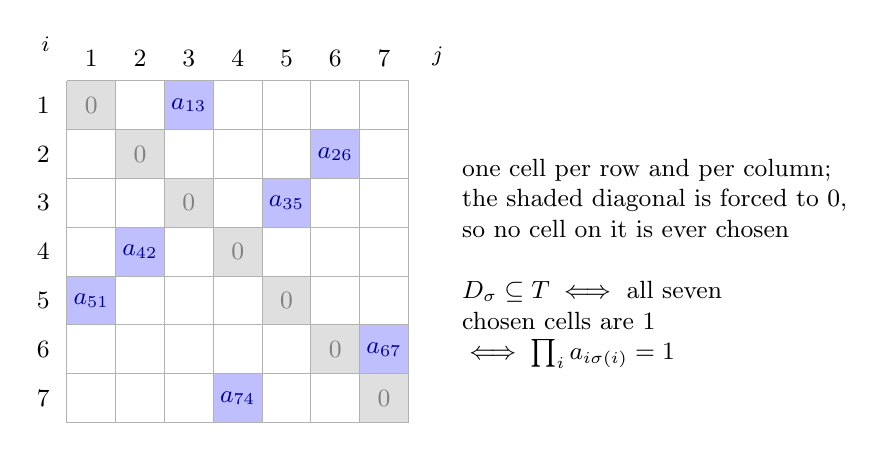
\begin{tikzpicture}[scale=0.62, every node/.style={font=\small}]
        \foreach \i in {1,...,7} \fill[gray!25] (\i-1,7-\i) rectangle (\i,8-\i);
        \foreach \i/\j in {1/3,2/6,3/5,4/2,5/1,6/7,7/4}
            \fill[blue!25] (\j-1,7-\i) rectangle (\j,8-\i);
        \draw[gray!60, thin] (0,0) grid (7,7);
        \foreach \i in {1,...,7} \node[anchor=east] at (-0.15,7.5-\i) {$\i$};
        \foreach \j in {1,...,7} \node[anchor=south] at (\j-0.5,7.1) {$\j$};
        \node[anchor=east, font=\footnotesize] at (-0.15,7.75) {$i$};
        \node[anchor=south, font=\footnotesize] at (7.6,7.1) {$j$};
        \foreach \i/\j in {1/3,2/6,3/5,4/2,5/1,6/7,7/4}
            \node[blue!60!black] at (\j-0.5,7.5-\i) {$a_{\i\j}$};
        \foreach \i in {1,...,7} \node[gray] at (\i-0.5,7.5-\i) {$0$};
        \node[anchor=west, align=left] at (7.9,4.6)
            {one cell per row and per column;\\the shaded diagonal is forced to \(0\),\\so no cell on it is ever chosen};
        \node[anchor=west, align=left] at (7.9,2.0)
            {\(D_\sigma \subseteq T \iff\) all seven\\chosen cells are \(1\)\\\(\iff \prod_{i} a_{i\sigma(i)} = 1\)};
    \end{tikzpicture}
\end{center}

Summing this indicator over all \(\sigma\) is exactly the following classical quantity.

\begin{definition}[Permanent]\label{def:permanent}
    For an \(n \times n\) matrix \(A\),
    \[
        \perm(A) = \sum_{\sigma \in S_n} \prod_{i=1}^{n} a_{i\sigma(i)}.
    \]
\end{definition}

\begin{lemma}\label{lem:F-is-permanent}
    \(F(T) = \perm(A)\).
\end{lemma}

\begin{proof}
    By \autoref{lem:perm-cycle-cover}, the subgraphs counted by \(F(T)\) are exactly the \(D_\sigma\) with \(\sigma \in S_n\) that happen to be subgraphs of \(T\), each arising from one \(\sigma\). Since every \(a_{ij} \in \{0,1\}\),
    \[
        D_\sigma \subseteq T
        \iff a_{i\sigma(i)} = 1 \ \forall\, i
        \iff \prod_{i=1}^{n} a_{i\sigma(i)} = 1,
    \]
    and the product is \(0\) for every other \(\sigma\). So the product is the indicator of \(\{D_\sigma \subseteq T\}\), and summing it over \(S_n\) counts the cycle covers of \(T\):
    \[
        F(T) = \sum_{\sigma \in S_n} \prod_{i=1}^{n} a_{i\sigma(i)} = \perm(A). \qedhere
    \]
\end{proof}

\begin{remark}
    The permutations contributing to \(\perm(A)\) have no fixed points, since \(a_{ii} = 0\), and no \(2\)-cycles, since \(a_{ij} a_{ji} = 0\) for \(i \ne j\) in a tournament. So all cycles of a cycle cover have length \(\ge 3\), as they must.
\end{remark}

The permanent differs from the determinant
\[
    \det(A) = \sum_{\sigma \in S_n} \sgn(\sigma) \prod_{i=1}^{n} a_{i\sigma(i)}
\]
only in the signs, yet the two behave completely differently: \(\det(A)\) is computable in \(O(n^3)\) steps by Gaussian elimination, because row operations are available, while computing \(\perm(A)\) exactly is \(\# \P\)-hard even for \(\{0,1\}\) matrices (Valiant, 1979). So we should not expect a formula for \(F(T)\). Fortunately we do not need one: an upper bound on \(\perm(A)\) in terms of the row sums of \(A\) will do, and those row sums are the out-degrees of \(T\), which sum to \(\binom{n}{2}\).

\subsection{Br\'egman's Theorem}

So far the chain of inequalities reads
\[
    C(T) \le F(T) = \perm(A), \qquad A = A_T \text{ the adjacency matrix of } T,
\]
and the tournament has disappeared: what is left is a question about \(\{0,1\}\) matrices.

\begin{question}\label{q:permanent}
    How large can the permanent of an \(n \times n\) matrix over \(\{0,1\}\) be?
\end{question}

Let \(r_i = \sum_{j=1}^{n} a_{ij}\) be the number of \(1\)s in the \(i\)-th row. A permutation \(\sigma\) contributing to \(\perm(A)\) must pick a \(1\) in every row, and there are \(r_i\) choices in row \(i\), so
\[
    \perm(A) \le r_1 r_2 \cdots r_n.
\]
This overcounts badly, because the choices in different rows may land in the same column, and then they do not form a permutation at all. The following theorem quantifies exactly how much is lost.

\begin{theorem}[Minc's conjecture, 1963; Br\'egman, 1973]\label{thm:bregman}
    For any \(n \times n\) matrix \(A\) over \(\{0,1\}\) with row sums \(r_i = \sum_{j=1}^{n} a_{ij}\),
    \[
        \perm(A) \le \prod_{i=1}^{n} (r_i!)^{1/r_i}.
    \]
\end{theorem}

\begin{remark}\hfill
    \begin{enumerate}[(1)]
        \item This is sharper than the trivial bound: \(r_i! \le r_i^{\,r_i}\) gives \((r_i!)^{1/r_i} \le r_i\). The gain per row is roughly a factor \(e\), since \((r!)^{1/r} \approx r/e\).
        \item A row with \(r_i = 0\) forces \(\perm(A) = 0\), so we may assume \(r_i \ge 1\) throughout.
        \item The bound is best possible: let \(A\) be block diagonal with all-\(1\) blocks of sizes \(d_1, \ldots, d_m\), where \(d_1 + \cdots + d_m = n\). A permutation contributes iff it preserves each block, so \(\perm(A) = \prod_{j} d_j!\); and every row inside the \(j\)-th block has \(r_i = d_j\), so \(\prod_i (r_i!)^{1/r_i} = \prod_j \bigl( (d_j!)^{1/d_j} \bigr)^{d_j} = \prod_j d_j!\) as well.
        \begin{center}
            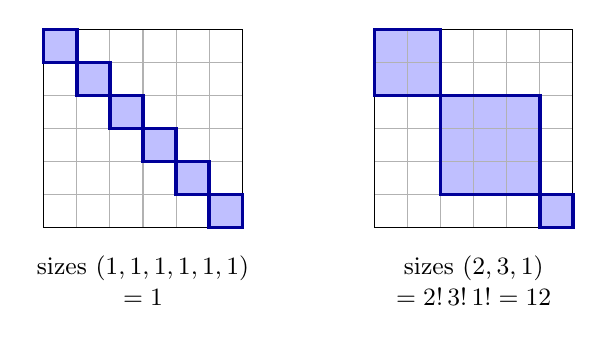
\begin{tikzpicture}[scale=0.42, every node/.style={font=\small}]
                % left: identity, all blocks of size 1
                \foreach \i in {1,...,6} \fill[blue!25] (\i-1,6-\i) rectangle (\i,7-\i);
                \draw[gray!60, thin] (0,0) grid (6,6);
                \draw (0,0) rectangle (6,6);
                \foreach \i in {1,...,6}
                    \draw[blue!60!black, very thick] (\i-1,6-\i) rectangle (\i,7-\i);
                \node[align=center] at (3,-1.6) {sizes $(1,1,1,1,1,1)$\\$\perm = 1$};
                % right: blocks of sizes 2, 3, 1
                \begin{scope}[xshift=10cm]
                    \fill[blue!25] (0,4) rectangle (2,6);
                    \fill[blue!25] (2,1) rectangle (5,4);
                    \fill[blue!25] (5,0) rectangle (6,1);
                    \draw[gray!60, thin] (0,0) grid (6,6);
                    \draw (0,0) rectangle (6,6);
                    \draw[blue!60!black, very thick] (0,4) rectangle (2,6);
                    \draw[blue!60!black, very thick] (2,1) rectangle (5,4);
                    \draw[blue!60!black, very thick] (5,0) rectangle (6,1);
                    \node[align=center] at (3,-1.6) {sizes $(2,3,1)$\\$\perm = 2!\,3!\,1! = 12$};
                \end{scope}
            \end{tikzpicture}
        \end{center}
    \end{enumerate}
\end{remark}

\subsection{Balancing the Out-Degrees}

We apply \autoref{thm:bregman} to the adjacency matrix of a tournament. There \(r_i\) is the out-degree of the \(i\)-th vertex, and since every edge of \(K_n\) is oriented exactly once,
\[
    \sum_{i=1}^{n} r_i = e(T) = \binom{n}{2}.
\]
This is the only information we have about the \(r_i\), so we must maximise the Br\'egman bound subject to it.

\begin{question}\label{q:balance}
    Given \(n\) and \(S\), if \(r_1 + \cdots + r_n = S\) with all \(r_i \ge 1\), how big can \(\prod_{i=1}^{n} (r_i!)^{1/r_i}\) be?
\end{question}

\begin{claim}\label{clm:balanced}
    The product is maximised when the \(r_i\) are as equal as possible, i.e.\ when every \(r_i\) is \(\lfloor \frac{S}{n} \rfloor\) or \(\lceil \frac{S}{n} \rceil\).
\end{claim}

\begin{proof}
    Write \(g(x) = (x!)^{1/x}\) for \(x \ge 1\). It suffices to show that if two of the \(r_i\) are \(a\) and \(b\) with \(a \le b - 2\), then replacing them by \(a+1\) and \(b-1\) strictly increases the product, i.e.
    \[
        g(a) \, g(b) < g(a+1) \, g(b-1)
        \iff \frac{g(a)}{g(a+1)} < \frac{g(b-1)}{g(b)}.
    \]
    So with \(f(x) \coloneqq \dfrac{g(x)}{g(x+1)}\) it is enough that \(f\) is strictly increasing, since \(a \le b-2 < b-1\).

    Fix \(x \ge 2\). Then
    \[
        f(x-1) < f(x)
        \iff g(x-1) \, g(x+1) < g(x)^2
        \iff \bigl( (x-1)! \bigr)^{\frac{1}{x-1}} \bigl( (x+1)! \bigr)^{\frac{1}{x+1}} < (x!)^{\frac{2}{x}}.
    \]
    Raise both sides to the power \(x(x-1)(x+1) > 0\) and substitute \((x-1)! = \frac{x!}{x}\) and \((x+1)! = (x+1) \cdot x!\):
    \[
        \Bigl( \frac{x!}{x} \Bigr)^{x(x+1)} \bigl( (x+1) \, x! \bigr)^{x(x-1)} < (x!)^{2(x^2-1)}
        \iff (x!)^{2x^2} \frac{(x+1)^{x(x-1)}}{x^{x(x+1)}} < (x!)^{2x^2 - 2},
    \]
    i.e.
    \[
        \Bigl( \frac{x+1}{x} \Bigr)^{x(x-1)} < \Bigl( \frac{x^x}{x!} \Bigr)^{2}. \tag{$\ast$}
    \]
    Now AM--GM applied to \(x! = 1 \cdot 2 \cdots x\) gives
    \[
        x! \le \Bigl( \frac{1 + 2 + \cdots + x}{x} \Bigr)^{x} = \Bigl( \frac{x+1}{2} \Bigr)^{x}
        \implies \Bigl( \frac{x^x}{x!} \Bigr)^{2} \ge \Bigl( \frac{2x}{x+1} \Bigr)^{2x} = 4^x \Bigl( \frac{x}{x+1} \Bigr)^{2x},
    \]
    so the ratio of the two sides of \((\ast)\) is
    \[
        \frac{(x^x/x!)^2}{\bigl( \frac{x+1}{x} \bigr)^{x(x-1)}}
        \ \ge\ 4^x \Bigl( \frac{x}{x+1} \Bigr)^{2x + x(x-1)}
        = 4^x \Bigl( \frac{x}{x+1} \Bigr)^{x(x+1)}
        = \Bigl[ 4 \Bigl( 1 - \frac{1}{x+1} \Bigr)^{x+1} \Bigr]^{x}.
    \]
    As \(x \ge 2\) we have \(x + 1 \ge 3\), and \(m \mapsto (1 - \frac{1}{m})^m\) is increasing,\footnote{It increases to \(e^{-1}\), so it is always \emph{below} \(e^{-1}\) and \(e^{-1}\) cannot be used as a lower bound here; any constant beating \(\frac{1}{4}\) suffices, and \(\frac{8}{27}\) does.} so \((1 - \frac{1}{x+1})^{x+1} \ge (\frac{2}{3})^3 = \frac{8}{27} > \frac{1}{4}\) and the bracket exceeds \(1\). Hence \((\ast)\) holds and \(f\) is strictly increasing.
\end{proof}

\begin{lemma}\label{lem:perm-tournament}
    There is an absolute constant \(c_1 > 0\) s.t.\ every \(n\)-vertex tournament \(T\) satisfies
    \[
        C(T) \le F(T) = \perm(A) \le c_1 \sqrt{n} \cdot \frac{n!}{2^n}.
    \]
\end{lemma}

\begin{proof}
    The out-degrees satisfy \(\sum_i r_i = \binom{n}{2}\), with average \(\frac{n-1}{2}\), so by \autoref{clm:balanced} the Br\'egman bound is largest when every \(r_i\) is \(\lfloor \frac{n-1}{2} \rfloor\) or \(\lceil \frac{n-1}{2} \rceil\). Also \(g(x) = (x!)^{1/x}\) is increasing, since
    \[
        g(x)^{x(x+1)} = (x!)^{x+1} \le (x!)^{x} (x+1)^x = \bigl( (x+1)! \bigr)^{x} = g(x+1)^{x(x+1)},
    \]
    so bounding every factor by the larger one gives, with \(R = \lceil \frac{n-1}{2} \rceil \le \frac{n}{2}\),
    \[
        \perm(A) \le \prod_{i=1}^{n} (r_i!)^{1/r_i} \le \bigl( (R!)^{1/R} \bigr)^{n}.
    \]
    Stirling's formula in the form \(R! = \sqrt{2\pi R} \, (\frac{R}{e})^{R} e^{\theta/(12R)}\) with \(0 < \theta < 1\) gives
    \[
        \bigl( (R!)^{1/R} \bigr)^{n} = \Bigl( \frac{R}{e} \Bigr)^{n} (2\pi R)^{\frac{n}{2R}} e^{\frac{\theta n}{12 R^2}}.
    \]
    Here \(\frac{n}{2R} \le \frac{n}{n-1} \le 2\) for \(n \ge 2\), so \((2\pi R)^{n/(2R)} \le (\pi n)^{n/(n-1)} = O(n)\), and \(e^{\theta n/(12R^2)} = e^{O(1/n)} = O(1)\). Hence
    \[
        \perm(A) \le O(n) \cdot \Bigl( \frac{n}{2e} \Bigr)^{n},
    \]
    and Stirling once more, now for \(n!\), turns \(\bigl( \frac{n}{2e} \bigr)^n = \frac{1}{2^n} \bigl( \frac{n}{e} \bigr)^n = (1 + o(1)) \frac{n!}{\sqrt{2\pi n} \, 2^n}\) into
    \[
        \perm(A) \le O(n) \cdot O\Bigl( \frac{n!}{\sqrt{n} \, 2^n} \Bigr) = O\Bigl( \sqrt{n} \cdot \frac{n!}{2^n} \Bigr). \qedhere
    \]
\end{proof}

\subsection{Proof of Alon's Theorem}

Collecting what we have, every \(n\)-vertex tournament satisfies
\[
    C(T) \le F(T) = \perm(A_T) \le c_1 \sqrt{n} \cdot \frac{n!}{2^n}
    \qquad \text{and} \qquad
    n \cdot C(T) \le P(T).
\]
The second inequality points the wrong way: it bounds cycles by paths, whereas we want to bound paths. The fix is to turn the paths of \(T\) into cycles by adding one vertex, and this is done at random, exactly as in \autoref{prop:szele-lower}.

\begin{proof}[Proof of \autoref{thm:alon-hamilton}]
    Let \(T\) be an \(n\)-vertex tournament. Construct a random tournament \(T^* \supseteq T\) on \(n+1\) vertices by adding a new vertex \(y\) and orienting each of the \(n\) edges at \(y\) uniformly at random, independently of each other.
    \begin{center}
        \begin{tikzpicture}[thick, >={Stealth[length=5pt]}, every node/.style={font=\small}]
            \draw[fill=blue!6] (0,0) ellipse (1.25 and 1.5);
            \node at (0,0) {$T$};
            \fill[red!80!black] (3.6,0) circle (2.6pt);
            \node[right=3pt, red!80!black] at (3.6,0) {$y$};
            \draw[->, red!80!black, shorten >=4pt] (3.6,0) to[out=160, in=20] (0.9,0.95);
            \draw[<-, red!80!black, shorten <=4pt] (3.6,0) to[out=180, in=0] (1.2,0.3);
            \draw[->, red!80!black, shorten >=4pt] (3.6,0) to[out=200, in=-20] (0.9,-0.95);
            \draw[<-, red!80!black, shorten <=4pt] (3.6,0) to[out=190, in=-5] (1.1,-0.4);
            \node[anchor=west, align=left] at (4.6,0)
                {each of the \(n\) edges at \(y\)\\is oriented by a fair coin,\\independently};
        \end{tikzpicture}
    \end{center}

    Every Hamilton cycle of \(T^*\) passes through \(y\), and deleting \(y\) from it leaves a Hamilton path of \(T\). Conversely, a Hamilton path \(v_1 \to \cdots \to v_n\) of \(T\) closes up into a Hamilton cycle of \(T^*\) exactly when \((v_n, y) \in E(T^*)\) and \((y, v_1) \in E(T^*)\), which are two of the \(n\) independent coin flips, so this happens with probability \(\frac{1}{4}\). Writing \(C(T^*)\) as a sum of indicators over the \(P(T)\) Hamilton paths of \(T\), linearity of expectation gives
    \[
        \mathbb{E}\bigl[ C(T^*) \bigr] = \sum_{\text{Hamilton paths of } T} \mathbb{P}(\text{the path closes up}) = \frac{P(T)}{4}.
    \]
    By \autoref{lem:first-moment} some outcome \(T^*\) has \(C(T^*) \ge \frac{P(T)}{4}\). Applying \autoref{lem:perm-tournament} to this \((n+1)\)-vertex tournament,
    \[
        \frac{P(T)}{4} \le C(T^*) \le c_1 \sqrt{n+1} \cdot \frac{(n+1)!}{2^{n+1}}
        \implies P(T) \le 2 c_1 (n+1)^{3/2} \cdot \frac{n!}{2^{n}} = c_1 (n+1)^{3/2} \cdot \frac{n!}{2^{n-1}},
    \]
    using \((n+1)! = (n+1) \cdot n!\). As \((n+1)^{3/2} \le (2n)^{3/2}\), this is at most \(c \, n^{3/2} \frac{n!}{2^{n-1}}\) with \(c = 2^{3/2} c_1\), and taking the maximum over \(T\) gives the theorem.
\end{proof}

\begin{remark}
    It is worth seeing where the polynomial factor \(n^{3/2}\) comes from: \(\sqrt{n}\) is the Stirling factor in \autoref{lem:perm-tournament}, and the extra \(n\) is the price of the one added vertex, \((n+1)! = (n+1) \cdot n!\). So Szele's conjecture is settled: by \autoref{prop:szele-lower} and \autoref{thm:alon-hamilton},
    \[
        \frac{n!}{2^{n-1}} \le P(n) \le c \, n^{3/2} \cdot \frac{n!}{2^{n-1}},
    \]
    and the random tournament of \autoref{prop:szele-lower} is optimal up to the factor \(n^{3/2}\).
\end{remark}

\section{Max-Cut}\label{sec:max-cut}

The next application of linearity is shorter, and the random object is a partition of the vertex set rather than a random graph.

\begin{question}\label{q:max-cut}
    Given a graph \(G\), how large a bipartite subgraph can we find inside it?
\end{question}

\begin{definition}[Cut]\label{def:cut}
    A \vocab{cut} of \(G\) is a partition \(V(G) = V_1 \cupdot V_2\). An edge is \vocab{crossing} if its two endpoints lie in different parts, and the \vocab{size} of the cut is the number of crossing edges.
\end{definition}

The crossing edges of a cut form a bipartite subgraph of \(G\), and conversely every bipartite subgraph arises this way, so \autoref{q:max-cut} asks for the largest cut, the \vocab{max-cut} of \(G\).

\subsection{Half of the Edges}

\begin{proposition}\label{prop:max-cut-half}
    Every graph \(G\) contains a bipartite subgraph with at least \(\frac{1}{2} e(G)\) edges.
\end{proposition}

\begin{proof}
    Take a uniformly random partition \(V(G) = V_1 \cupdot V_2\), i.e.\ put each vertex into \(V_1\) or \(V_2\) by an independent fair coin, and keep all crossing edges. Let \(X\) be the number of crossing edges, so that
    \[
        X = \sum_{e \in E(G)} \mathbbm{1}_{\{e \text{ is crossing}\}}.
    \]
    For a fixed edge \(e = uv\), the four placements of \(u\) and \(v\) are equally likely and two of them separate the endpoints, so \(\mathbb{P}(e \text{ is crossing}) = \frac{1}{2}\). By \autoref{thm:linearity},
    \[
        \mathbb{E}[X] = \sum_{e \in E(G)} \mathbb{P}(e \text{ is crossing}) = \sum_{e \in E(G)} \frac{1}{2} = \frac{1}{2} e(G),
    \]
    and by \autoref{lem:first-moment} some partition achieves at least this many crossing edges.
\end{proof}

The same bound has a second proof, with no randomness at all, which is worth comparing: instead of averaging over all cuts, it starts at the best cut and perturbs it.

\begin{proof}[Second proof of \autoref{prop:max-cut-half}]
    Take a \emph{maximum} cut \(V = V_1 \cupdot V_2\).

    \begin{claim}
        Every vertex sends at least half of its edges across the cut.
    \end{claim}
    \begin{subproof}
        If some \(v\) sent more than half of its edges inside its own part, moving \(v\) to the other part would turn all of those into crossing edges and only lose the ones it already had crossing, strictly increasing the size of the cut, contradicting maximality.
    \end{subproof}
    \begin{center}
        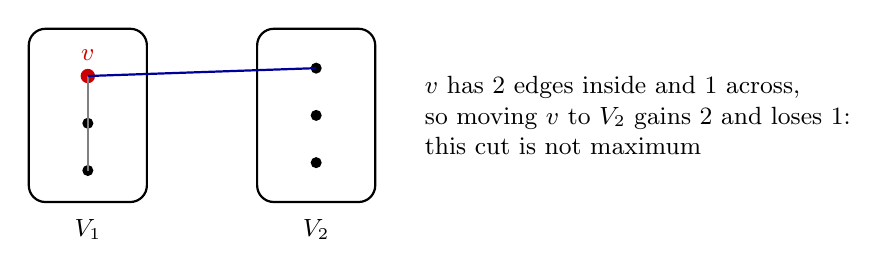
\begin{tikzpicture}[thick, every node/.style={font=\small}]
            \draw[rounded corners=6pt] (-1.5,-1.1) rectangle (0.0,1.1);
            \draw[rounded corners=6pt] (1.4,-1.1) rectangle (2.9,1.1);
            \node at (-0.75,-1.45) {$V_1$};
            \node at (2.15,-1.45) {$V_2$};
            \fill[red!80!black] (-0.75,0.5) circle (2.6pt);
            \node[above=2pt, red!80!black] at (-0.75,0.5) {$v$};
            \foreach \y in {-0.1,-0.7} \fill (-0.75,\y) circle (2pt);
            \foreach \y in {0.6,0.0,-0.6} \fill (2.15,\y) circle (2pt);
            \foreach \y in {-0.1,-0.7} \draw[gray] (-0.75,0.5) -- (-0.75,\y);
            \draw[blue!60!black] (-0.75,0.5) -- (2.15,0.6);
            \node[anchor=west, align=left] at (3.4,0)
                {\(v\) has \(2\) edges inside and \(1\) across,\\so moving \(v\) to \(V_2\) gains \(2\) and loses \(1\):\\this cut is not maximum};
        \end{tikzpicture}
    \end{center}
    Summing the claim over all vertices, each crossing edge being counted twice,
    \[
        2 \cdot \#\{\text{crossing edges}\} = \sum_{v \in V} \#\{\text{crossing edges at } v\} \ge \sum_{v \in V} \frac{d(v)}{2} = e(G). \qedhere
    \]
\end{proof}

\subsection{Beating One Half}

\begin{remark}\label{rmk:half-tight}
    The constant \(\frac{1}{2}\) cannot be improved, as \(G = K_n\) shows. Its largest bipartite subgraph is \(K_{\lceil n/2 \rceil, \lfloor n/2 \rfloor}\), with \(\lfloor \frac{n^2}{4} \rfloor\) edges, while \(e(K_n) = \binom{n}{2} = \frac{n(n-1)}{2}\), and
    \[
        \frac{\lfloor n^2/4 \rfloor}{\binom{n}{2}} \longrightarrow \frac{1}{2}.
    \]
\end{remark}

The ratio tends to \(\frac{1}{2}\) but is never equal to it: for \(n = 2k\) it is \(\frac{k^2}{k(2k-1)} = \frac{k}{2k-1}\). So there should be room for an improvement of \autoref{prop:max-cut-half} by a term depending on \(n\), and there is. The proof is the same one-line computation, with one change: the random partition is taken to be \emph{balanced}, which makes an edge slightly more likely to cross.

\begin{theorem}\label{thm:max-cut-sharp}
    Let \(G\) be a graph on \(n\) vertices. Then \(G\) has a bipartite subgraph with at least
    \[
        e(G) \cdot \frac{k}{2k-1} \quad \text{edges if } n = 2k,
        \qquad
        e(G) \cdot \frac{k+1}{2k+1} \quad \text{edges if } n = 2k+1.
    \]
\end{theorem}

\begin{proof}
    Take \(V = V_1 \cupdot V_2\) where \(V_1\) is a uniformly random subset of exactly \(k\) vertices, and let \(X\) be the number of crossing edges. For a fixed edge \(e = uv\), the pair \((u,v)\) is equally likely to be any ordered pair of distinct vertices, so
    \[
        \mathbb{P}(e \text{ is crossing}) = 2 \cdot \frac{\abs{V_1}}{n} \cdot \frac{\abs{V_2}}{n-1} =
        \begin{cases}
            2 \cdot \dfrac{k}{2k} \cdot \dfrac{k}{2k-1} = \dfrac{k}{2k-1}, & n = 2k, \\[2ex]
            2 \cdot \dfrac{k}{2k+1} \cdot \dfrac{k+1}{2k} = \dfrac{k+1}{2k+1}, & n = 2k+1.
        \end{cases}
    \]
    By \autoref{thm:linearity}, \(\mathbb{E}[X] = e(G) \cdot \mathbb{P}(e \text{ is crossing})\), and \autoref{lem:first-moment} gives a partition attaining it.
\end{proof}

\begin{remark}
    Both bounds are exactly tight for \(K_n\), by \autoref{rmk:half-tight}: for \(n = 2k\), \(e(K_n) \cdot \frac{k}{2k-1} = k(2k-1) \cdot \frac{k}{2k-1} = k^2\), and for \(n = 2k+1\), \(e(K_n) \cdot \frac{k+1}{2k+1} = k(2k+1) \cdot \frac{k+1}{2k+1} = k(k+1)\). Writing the two factors as \(\frac{1}{2} + \frac{1}{2(n-1)}\) and \(\frac{1}{2} + \frac{1}{2n}\) shows how much is gained over \autoref{prop:max-cut-half}, and that the gain vanishes as \(n\) grows.
\end{remark}

\section{Counting Monochromatic Cliques}\label{sec:ramsey-counting}

The last application of this chapter returns to where the course began, the Ramsey number \(R(k)\) of \autoref{def:ramsey-number}. Erd\H{o}s's lower bound \autoref{thm:erdos-ramsey} was proved by a union bound; we now redo it as a first moment computation, which gives a stronger conclusion for free, and then ask what happens for hypergraphs.

\subsection{The Erd\H{o}s Bound Revisited}

\begin{lemma}\label{lem:count-mono}
    For any \(n\) and \(t\), there is a red/blue coloring of \(E(K_n)\) with at most \(\binom{n}{t} 2^{1 - \binom{t}{2}}\) monochromatic copies of \(K_t\).
\end{lemma}

\begin{proof}
    Color the edges uniformly at random, independently, and let \(X\) be the number of monochromatic copies of \(K_t\). Indexing by the vertex set of the copy,
    \[
        X = \sum_{S \in \binom{V}{t}} \mathbbm{1}_{\{S \text{ spans a monochromatic clique}\}}.
    \]
    A fixed \(S\) spans \(\binom{t}{2}\) edges, all of which must receive the same one of two colors, so
    \[
        \mathbb{P}(S \text{ is monochromatic}) = 2 \cdot 2^{-\binom{t}{2}}.
    \]
    By \autoref{thm:linearity},
    \[
        \mathbb{E}[X] = \sum_{S \in \binom{V}{t}} \mathbb{P}(S \text{ is monochromatic}) = \binom{n}{t} 2^{1 - \binom{t}{2}},
    \]
    and by \autoref{lem:first-moment} some coloring has at most this many monochromatic copies.
\end{proof}

\begin{corollary}\label{cor:ramsey-lower}
    If \(\binom{n}{t} 2^{1-\binom{t}{2}} < 1\), then \(R(t) > n\). Consequently \(R(t) \ge \sqrt{2}^{\,(1-o(1))t}\).
\end{corollary}

\begin{proof}
    The number of monochromatic copies is an integer, so the coloring of \autoref{lem:count-mono} has none at all, and \(K_n\) has a coloring without a monochromatic \(K_t\). The estimate \(\binom{n}{t} 2^{1-\binom{t}{2}} < 2 n^t 2^{-t(t-1)/2}\) is \(< 1\) as soon as \(n \le (1-c) 2^{(t-1)/2}\), exactly as in \autoref{thm:erdos-ramsey}.
\end{proof}

\begin{remark}
    \autoref{lem:count-mono} says strictly more than the union bound of \autoref{thm:erdos-ramsey}: it gives a coloring with \emph{few} monochromatic cliques even when the expectation is much larger than \(1\), whereas the union bound is silent as soon as the sum of probabilities reaches \(1\). Compare \autoref{eg:union-bound-expectation}.
\end{remark}

\subsection{Hypergraph Ramsey Numbers}

\begin{question}
    What happens for \(k\)-uniform hypergraphs?
\end{question}

Two-color the \(k\)-element edges \(\binom{[n]}{k}\) of the complete \(k\)-uniform hypergraph \(K_n^{(k)}\), and look for a set \(S\) of \(t\) vertices all of whose \(\binom{t}{k}\) edges have the same color.

\begin{definition}\label{def:hypergraph-ramsey}
    The \vocab{\(k\)-uniform Ramsey number} \(R^{(k)}(t)\) is the smallest \(n\) s.t.\ every red/blue coloring of \(\binom{[n]}{k}\) contains a monochromatic set of \(t\) vertices. So \(R^{(2)}(t) = R(t)\).
\end{definition}

\begin{remark}
    A \(t\)-set of vertices spans \(\binom{t}{2}\) graph edges but \(\binom{t}{k} \gg \binom{t}{2}\) hypergraph edges, so there are far more constraints to violate and it is correspondingly easier to make a \(t\)-set non-monochromatic. We should therefore expect \(R^{(k)}(t) \gg R(t)\), and indeed each extra level of uniformity costs an exponential.
\end{remark}

What is known is a tower of exponentials, of height \(k-2\) from below and \(k-1\) from above, for some constant \(c > 0\):
\[
    \sqrt{2}^{\,t} \le R(t) \le 4^t, \qquad
    c^{\,t} \le R^{(3)}(t) \le 2^{c^{\,t}}, \qquad
    2^{c^{\,t}} \le R^{(4)}(t) \le 2^{2^{c^{\,t}}}, \qquad \ldots
\]
Already for \(k = 3\) the gap between the two sides is an entire exponential, and closing it is a well-known open problem. Instead of a monochromatic set one can ask for the weaker conclusion that some color is merely \emph{dominant} on a set, and then much larger sets can be found.

\begin{theorem}\label{thm:dominant-color}
    If we red/blue color the edges of \(K_n^{(k)}\), then there is a set \(S\) of \(\Omega\bigl( (\log n)^{1/(k-1)} \bigr)\) vertices on which some color appears on a \(\bigl( \frac{1}{2} + c_k \bigr)\)-proportion of the edges, for some constant \(c_k > 0\).
\end{theorem}

\begin{recall}
    There are colorings in which the largest monochromatic set has size only
    \[
        O(\underbrace{\log \log \cdots \log}_{k-2 \text{ times}} n).
    \]
\end{recall}

So the two conclusions live on completely different scales: insisting on \emph{all} edges of \(S\) having one color forces \(S\) to be tiny, while asking only for a fixed advantage over \(\frac{1}{2}\) allows \(S\) to be polylogarithmic in \(n\).
\begin{center}
    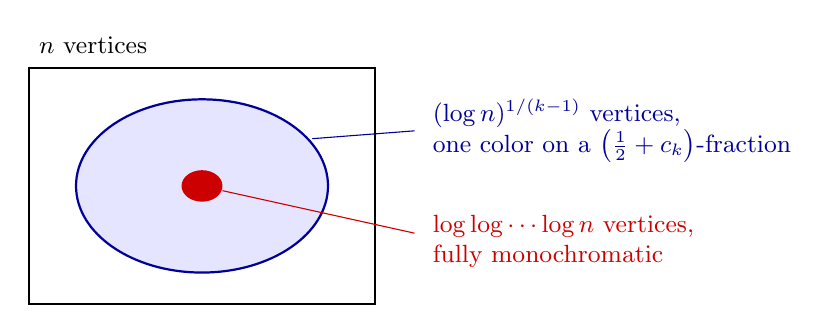
\begin{tikzpicture}[thick, every node/.style={font=\small}]
        \draw (0,0) rectangle (4.4,3.0);
        \node[anchor=south west] at (0,3.05) {$n$ vertices};
        \fill[blue!10] (2.2,1.5) ellipse (1.6 and 1.1);
        \draw[blue!60!black] (2.2,1.5) ellipse (1.6 and 1.1);
        \node[blue!60!black, anchor=west, align=left] at (5.0,2.2)
            {$(\log n)^{1/(k-1)}$ vertices,\\one color on a $\bigl( \frac{1}{2} + c_k \bigr)$-fraction};
        \fill[red!80!black] (2.2,1.5) ellipse (0.26 and 0.2);
        \node[red!80!black, anchor=west, align=left] at (5.0,0.8)
            {$\log \log \cdots \log n$ vertices,\\fully monochromatic};
        \draw[blue!60!black, thin] (3.6,2.1) -- (4.9,2.2);
        \draw[red!80!black, thin] (2.46,1.44) -- (4.9,0.9);
    \end{tikzpicture}
\end{center}
